\documentclass[a4paper]{article}

\usepackage{mhchem}%化学符号的宏包
\usepackage{cite}%多个文献引用
\usepackage{graphicx}
\usepackage{array}%调节表格行高
\usepackage{multirow,makecell}%多行表格
\usepackage{tabularx}%表格固定列宽
\usepackage{subfigure}
\usepackage{titlesec}%标题格式设置
\usepackage{amsmath}
\usepackage{amssymb}
\usepackage{tabularx}
\usepackage{makecell}
\usepackage{geometry}
\usepackage{float}
\usepackage{setspace}%行距包
\usepackage{siunitx}
\usepackage{mdwlist}
\usepackage{tabu}
\usepackage{enumerate}

\geometry{top=1.54cm,bottom=2.54cm,left=2.5cm,right=2.5cm}


\begin{document}
\begin{center}
\bf\Large
EE 105 Feedback Control Systems\par
Department of Electrical and Computer Engineering\par
Tufts University Fall 2018\par
Homework \#2\par   
\end{center}
\begin{table}[H]
\begin{center}
\begin{tabular*}{\textwidth}{@{\extracolsep{\fill}}lcr}
Name: {\it Shang Wang} &Student ID: {\it 1277417} &E-mail: {\it shang.wang@tufts.edu}\\
\hline
\end{tabular*}
\end{center}
\end{table}

\section{Problem 1}
{\bf Answer: }\\
(a) According to the problem statement.\\
$$
i_L + \frac{L}{R} \frac{{\rm d} i_L}{{\rm d}t} = I
$$
So Laplace transform:
$$
I_L(s) = I(\frac{1}{1+\frac RL s}) 
$$
Since $I = u(t)$ and $\mathcal{L} (u(t)) = 1/s$, $I_L$ becomes:
$$
I_L = \frac{1}{s}(\frac{1}{1+\frac RL s}) = \frac{L/R}{s^2 + (L/S) s}
$$
And the $i_L(t)$ is:
$$
\mathcal{L}^{-1}(I_L(s)) = u(t)(1-e^{-\frac LR t})
$$\\
(b) Using mathematica to draw the plot when $L = 75 \rm nH$ and $R = 50 \Omega$.
\begin{figure}[hbtp]
\centering
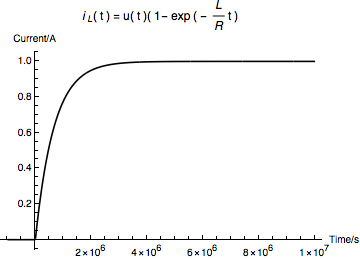
\includegraphics[width=0.6\textwidth]{pic/iLt.png}
\caption{Plot of $i_L(t)$} 
\label{iLt}
\end{figure}
We can see that the time constant $\tau = R/F = 6.7\times 10 ^{5}$, so it will take hours to reach the stable state.

\section{Problem 2}
{\bf Answer:}\\
(a) $e^{-t}-e^{-2t}$
We have:
$$
F(s) = \frac{1}{s+1}+\frac{1}{s+2}
$$
(b) $t^2$
We have:
$$
F(s) = \frac{2}{s^3}
$$
(c) $\cosh(3t)$
We have:
$$
F(s) = \frac{s}{s^2-9}
$$
(d) $t\cosh(3t)$
We have:
$$
F(s) = \frac{\rm d }{{\rm d}s}\mathcal{L}^{-1}(\cosh(3t)) = -\frac{s^2+9}{(s^2-9)^2}
$$
(e)$e{-2t}\cosh(3t)$
We have:
$$
F(s) = \frac{s+2}{(s+2)^2-9} = \frac{s+2}{s^2+4s-5}
$$
(f)$(2t)^2$
We have:
$$
F(s) = \frac12\frac{2}{(s/2)^3} = \frac{8}{s^3}
$$
(g)$(t-5)^2 u(t-5)$
We have:
$$
F(s) =\frac{2 e^{-5s}}{s^3}
$$

\section{Problem 3}
{\bf Answer: }\\
(a) According to the problem statement:
$$
F(s) = \frac{s}{(s+1)(s+4)} = \frac 13\Big(\frac{4}{s+4}-\frac{1}{s+1}\Big)
$$
which means:
$$
f(t) = \frac 13 u(t)(4e^{-4t}-e^{-t})
$$
(b) According to the problem statement:
$$
F(s) = \frac{s^3+6s^2+6s}{s^2+6s^+8} = s-\frac{2s}{s^2+6s+8}=s-2(\frac{2}{s+4}-\frac{1}{s+2})
$$
So the inverse Laplace transform is:
$$
f(t) = \delta'(t)-4e^{-4t}+2e^{-2t}
$$
(c) According to the problem statement:
$$
F(s) = \frac{s+1}{s^2+2s}= \frac{s+1}{s(s+2)} =\frac 12 (\frac{1}{s}+\frac{1}{s+2})
$$
So the inverse Laplace transform is:
$$
f(t) = \frac 12 u(t)(1+e^{-2t})
$$
(d)
According to the problem statement:
$$
F(s) = \frac{e^{-2s}}{(s+1)(s+2)^2} = e^{-2s}\Big(\frac{1}{s+1}-\frac{1}{s+2}-\frac{1}{(s+2)^2} \Big)
$$
Assume:
$$
F(s) = e^{-2s}F_1(s)
$$
We have:
$$
\mathcal{L}(F_1(s)) = u(t)(e^{-t}+e^{-2t}+te^{-2t})
$$
Then we get:
$$
f(t) = \mathcal{L}(F(s)) = \mathcal{L}(e^{-2s}F_1(s)) = u(t-2)(e^{-(t-2)}+e^{-2(t-2)}+te^{-2(t-2)})
$$
\section{Problem 4}
{\bf Answer: }\\
This block diagram is :
\begin{figure}[H]
\centering
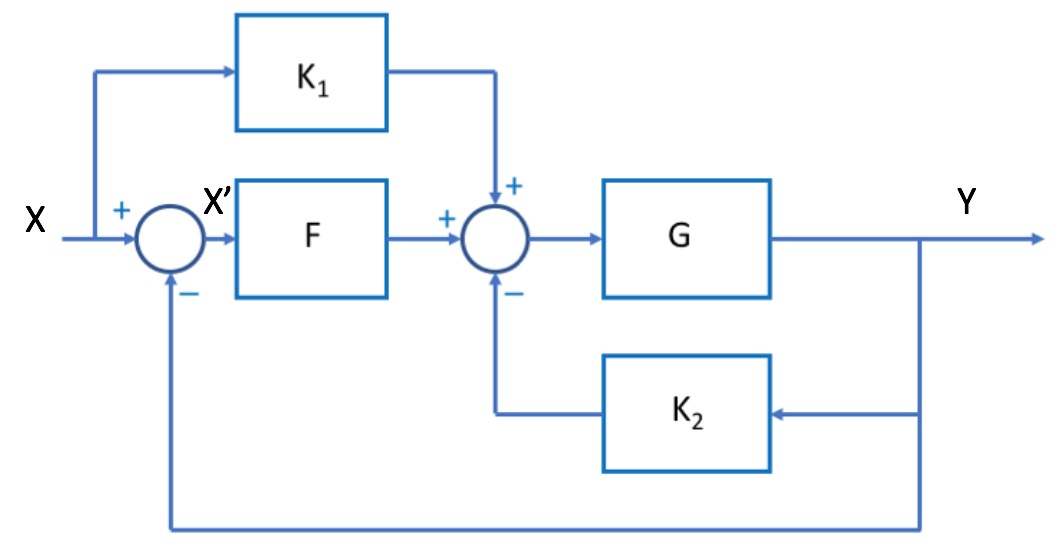
\includegraphics[width=0.6\textwidth]{pic/block.jpg}
\caption{The block diagram} 
\end{figure}


\noindent Where $X$ is the input of the system, and $Y$ is the output of the system.\\
Here we can use the Black's Formula to combine the $G$ and $K_2$.
$$
P = \frac{G}{1+GK_2}
$$
And we can list the following equations:
$$
X' = X-Y
$$
$$
Y = P(FX'+K_1X)
$$
Then we can figure out the relationship between $Y$ and $X$:
$$
\frac{Y}{X} = \frac{PF+PK_1}{1+PF} = \frac{G(F+K_1)}{1+G(F+K_2)}
$$
So the transfer function of the single block should be that.





\end{document}